\documentclass{article}

% if you need to pass options to natbib, use, e.g.:
%     \PassOptionsToPackage{numbers, compress}{natbib}
% before loading neurips_2018

% ready for submission
% \usepackage{neurips_2018}

% to compile a preprint version, e.g., for submission to arXiv, add add the
% [preprint] option:
\usepackage[preprint]{neurips_2019}

% to compile a camera-ready version, add the [final] option, e.g.:
     % \usepackage[final]{neurips_2019}

% to avoid loading the natbib package, add option nonatbib:
%     \usepackage[nonatbib]{neurips_2018}

\usepackage[utf8]{inputenc} % allow utf-8 input
\usepackage[T1]{fontenc}    % use 8-bit T1 fonts
\usepackage{hyperref}       % hyperlinks
\usepackage{url}            % simple URL typesetting
\usepackage{graphicx}
\usepackage{booktabs}       % professional-quality tables
\usepackage{amsfonts}       % blackboard math symbols
\usepackage{nicefrac}       % compact symbols for 1/2, etc.
\usepackage{microtype}      % microtypography
\usepackage{listings}
\usepackage{tabularx}
\usepackage{listings}
\usepackage{pgfplots}
\usepackage{tikz}
\usepackage{todonotes}
\usepackage{tikz-cd}
\usepackage{algorithm}
\usepackage{algpseudocode}
\usepackage{wrapfig}

\newcommand{\n}[1]{\ensuremath{n_{#1}}}
\newcommand{\rv}[1]{\ensuremath{{#1}_{1:n_{#1}}}}
\newcommand{\rvv}[1]{\ensuremath{{#1}_{1:n_{#1'}}}}
\newcommand{\model}[1]{\ensuremath{\mathcal{M}{(#1)}}}
\newcommand{\simu}[1]{\ensuremath{\Omega(\model{#1})}}
\newcommand{\micro}[2]{\ensuremath{\phi_{#1}(#2)}}
\newcommand{\pdf}[1]{\ensuremath{\mathcal{P}_{d}(#1)}}
\newcommand{\pmf}[1]{\ensuremath{\mathcal{P}_{m}(#1)}}
\newcommand{\add}[1]{\ensuremath{A_{#1}}}
\newcommand{\adds}[2]{\ensuremath{A_{#1}_{#2}}}
\newcommand{\expect}[1]{\ensuremath{\mathbb{E}[#1]}}
\newcommand{\trace}[1]{\ensuremath{\mathcal{T}_{#1}}}
\newcommand{\traces}[2]{\ensuremath{\textit{tr}^{#1}_{#2}}}
\newcommand{\stoc}[2]{\ensuremath{f^{#1}_{#2}(\rvv{x})}}
% \usepackage[binary-units=true]{siunitx}
\title{Hijacking Simulators with Universal Probabilistic Programming}

% neurlps classification
% Primary: Applications
% Secodnary cat:Data, Challenges, Implementations, and Software
% or Hijacking Malaria Simulators with Probabilistic Programming

% The \author macro works with any number of authors. There are two commands
% used to separate the names and addresses of multiple authors: \And and \AND.
%
% Using \And between authors leaves it to LaTeX to determine where to break the
% lines. Using \AND forces a line break at that point. So, if LaTeX puts 3 of 4
% authors names on the first line, and the last on the second line, try using
% \AND instead of \And before the third author name.
\newcommand{\bg}[1]{~{{[{\it \textcolor{red}{{\bf BG:} #1}}]}}}
\newcommand{\cs}[1]{~{{[{\it \textcolor{red}{{\bf CS:} #1}}]}}}
\newcommand{\ag}[1]{~{{[{\it \textcolor{red}{{\bf AG:} #1}}]}}}
% If accepted, instead use the following line for the camera-ready submission:
%\usepackage[accepted]{icml2019}
\usetikzlibrary{arrows,chains,matrix,positioning,scopes, arrows.meta}
\tikzset{
  shift left/.style ={commutative diagrams/shift left={#1}},
  shift right/.style={commutative diagrams/shift right={#1}}
}
\tikzset{%
  >={Latex[width=2mm,length=2mm]},
  % Specifications for style of nodes:
            base/.style = {rectangle, rounded corners, draw=black,
                           minimum width=4cm, minimum height=1cm,
                           text centered, font=\sffamily},
  activityStarts/.style = {base, fill=blue!50},
       startstop/.style = {base, fill=red!50},
    activityRuns/.style = {base, fill=green!50},
         process/.style = {base, minimum width=2.5cm, fill=orange!55,
                           font=\ttfamily},
}
\makeatletter
\tikzset{join/.code=\tikzset{after node path={%
\ifx\tikzchainprevious\pgfutil@empty\else(\tikzchainprevious)%
edge[every join]#1(\tikzchaincurrent)\fi}}}
\makeatother
%
\tikzset{>=stealth',every on chain/.append style={join},
         every join/.style={->}}
\tikzstyle{labeled}=[execute at begin node=$\scriptstyle,
   execute at end node=$]
   
\lstset{language=C++,
                basicstyle=\footnotesize,
                keywordstyle=\color{blue}\ttfamily,
                stringstyle=\color{red}\ttfamily,
                commentstyle=\color{green}\ttfamily,
                morecomment=[l][\color{magenta}]{\#},
                breaklines = true
}
\pgfplotsset{width=7cm,compat=1.8}
\author{%
Paper ID: }
  % examples of more authors
  % \And
  % Coauthor \\
  % Affiliation \\
  % Address \\
  % \texttt{email} \\
  % \AND
  % Coauthor \\
  % Affiliation \\
  % Address \\
  % \texttt{email} \\
  % \And
  % Coauthor \\
  % Affiliation \\
  % Address \\
  % \texttt{email} \\
  % \And
  % Coauthor \\
  % Affiliation \\
  % Address \\
  % \texttt{email} \\
%}
\begin{document}
% \nipsfinalcopy is no longer used

\maketitle

\begin{abstract}

% A goal of probabilistic programming is to couple simulators, with inference. This is 
% because stochastic simulators are used prominently in many industrial settings,
% do not require one to construct hand-crafted joint distributions as they implicitly 
% define a joint distribution of the program and encode learnt structures 
% directly. This makes simulators powerful tools and much of machine learning (ML) and 
% Artificial Intelligence (AI)
% can be seen as trying to emulate such simulators from a purely data-driven approach.
% However, in the 
% ML/AI setting, although we can often infer outcomes, we have little understanding about what 
% in the data led to the outputted inferences. 
% This makes it challenging to deploy ML/AI systems into the wild, especially in health-related and safety-critical domains, such
% as epidemiology, as we lose \emph{interpretability}. 
% In this work, we explain how to design ML/AI systems that combine
% probabilistic programming systems (PPSs) and epidemiology simulators, to extract
% fully interpretable posterior structures, enabling policy makers 
% and practitioners to make interpretable inferences. 
% In particular, we demonstrate this for the Malaria disease and show how we can 
% perform interpretable inference in such settings.

Probabilistic programming provides a way to perform statistical inference over simulations of events in a programmatic way. Thus, by design, simulators are ideal programs for probabilistic programming systems~(PPSs).
Simulators arise in a number of industrial scientific and industrial domains and encode sophisticated generative models.
However, within existing PPSs one would have to re-implement the simulator via the PPS language specification, which is inefficient and often not feasible due to the complexity of such scientific and industrial simulators.
Recent work by \cite{baydin2018efficient} demonstrated a pathway to turn a particular
type of event-based simulator into a probabilistic program, without having to re-implement the simulator in the existing PPS. 
% via the raw random number calls of the simulator.
 However, this still meant that a large class of critically important population-based simulators could not be turned into probabilistic programs and as such could not be used within a probabilistic programming framework.
In this work, we extend that framework to encompass population-based simulators, a very large class of simulators that are used extensively across epidemiology, multi-agent and financial modeling and provide the relevant
theoretical underpinnings. 
We enable simulators written in 13 different languages to be easily converted to probabilistic programs, for which we algorithmically outline and provide comprehensive examples of our system applied to a number of real-world population-based simulators.

% \todo[inline]{We need to have probabilistic programming in the title to make sure we attract the correct reviewers}

% Epidemiology simulations have become a fundamental tool in the fight
% against the epidemics of various infectious diseases like AIDS and
% malaria.
% However, the complicated and stochastic nature of these simulators
% can mean their output is difficult to interpret, which reduces their usefulness to policymakers.
% In this paper, we introduce an approach that allows one to treat a large class of population-based epidemiology simulators as probabilistic generative models.
%  This is achieved by \emph{hijacking} the internal random number generator calls, through the use of an universal probabilistic programming system (PPS). 
%  In contrast to other methods, our approach can be easily retrofitted to simulators written in popular industrial programming frameworks. 
% We demonstrate that our method can be used for interpretable introspection and inference, thus shedding light on black-box simulators. 
% This reinstates much needed trust between policymakers and evidence-based methods. 
\end{abstract}

\section{Introduction}
\label{sec:intro}
% \bg{The audience is a probabilistic programming audience - so that is what we will target}

% \begin{itemize}

% \item Talk about a goal of probabilistic programming is to simultaneously simulate and perform inference on models conditioned on the observations. Although universal probabilistic programming systems have the ability to do this, they are constrained because the simulator has to be re-written as a program inside that system; this is both infeasible for sufficiently large simulators and inefficient. It would however be much more efficient to turn simulators into probabilistic programs... then talk briefly about the foundations created by baydin et al. (2 paragraphs)
% \item Talk about the large body of simulators out there and briefly talk about the types of simulators
% i.e population-based, event-based, single-object based and so fourth. {1 paragraph}
% \item Talk, high level, about the notion of a posterior in terms of traces either add stuff from tom's thesis or directly cite. (1 paragraph)
% \item Talk about the experiments we perform (high- level)


% \end{itemize}


% One powerful \emph{class} of models are simulators. 
Simulators are useful tools when conducting experiments in the real system 
is impossible, or impractical and they arise in numerous industrial \cite{di2015simulator,judd2009numerically,kass1990rapid} and scientific applications~\cite{smith2008towards,bershteyn2018implementation,gleisberg_event_2008}. 
They are rich models and provide a level of interpretability not typically found in modern deep learning methodologies due to the several years, if not decades, of research and development that has led to their construction.
Thus, simulators by their very nature are information rich and naturally describe complicated joint densities.
That is the \emph{model}, or equivalently \emph{program}, specified by the simulator defines a joint density $p(x,y)$ and the inputs into the simulator denote priors $p(x)$. 
But, for all the benefits of using simulations there exist two challenging problems that are currently faced:
\begin{itemize}
\item It is difficult to calibrate the internal simulator parameters, as the events they are simulating are expensive to reproduce, or are very rare, so data is scarce. 
\item As the development process takes place over several years the code base becomes convoluted, making it increasingly challenging to understand the structure of the joint density and the internal operations within the simulator, diminishing the interpretability that the simulator once provided. 
\end{itemize}

One such machine learning paradigm that has the ability to resolve these issues is \emph{Probabilistic programming}\cite{gordon2014probabilistic,milch2005blog,van2018introduction,tran2017deep}. 
Probabilistic programming enables users to write, condition on and perform inference in, complex probabilistic models in a programmatic, yet efficient and simplified way. 
The source code of the given model, or equivalently the \emph{program}, is transformed into a program density, which can
be viewed as the joint density of the user-specified model, \emph{the simulator} in this instance.
Having direct access to the source code enables PPSs to conduct several processes automatically, such as 
the automation of complex statistical inference procedures\cite{zhou2019lf,goodman2012church,wood2014new,rainforth2017automating}, which enables us to efficiently calibrate
model parameters, and we can also track how the internals of the program change during
run time, enabling a full analysis of the program structure and traces generated\cite{milch2005blog}, which provides greater interpretability, see Figure~\ref{fig:hijacking}.
In addition to this, as models are directly expressed in program code we can encode other structures to make use of the full structure of a given language, whether that is \texttt{python, C++} or 
any other language,
which enables users to integrate PPSs into their standard model development process, increasing efficiency and reducing model iteration time.

\begin{wrapfigure}{R}{0.44\textwidth}
\vspace{-20pt}
\centering
% 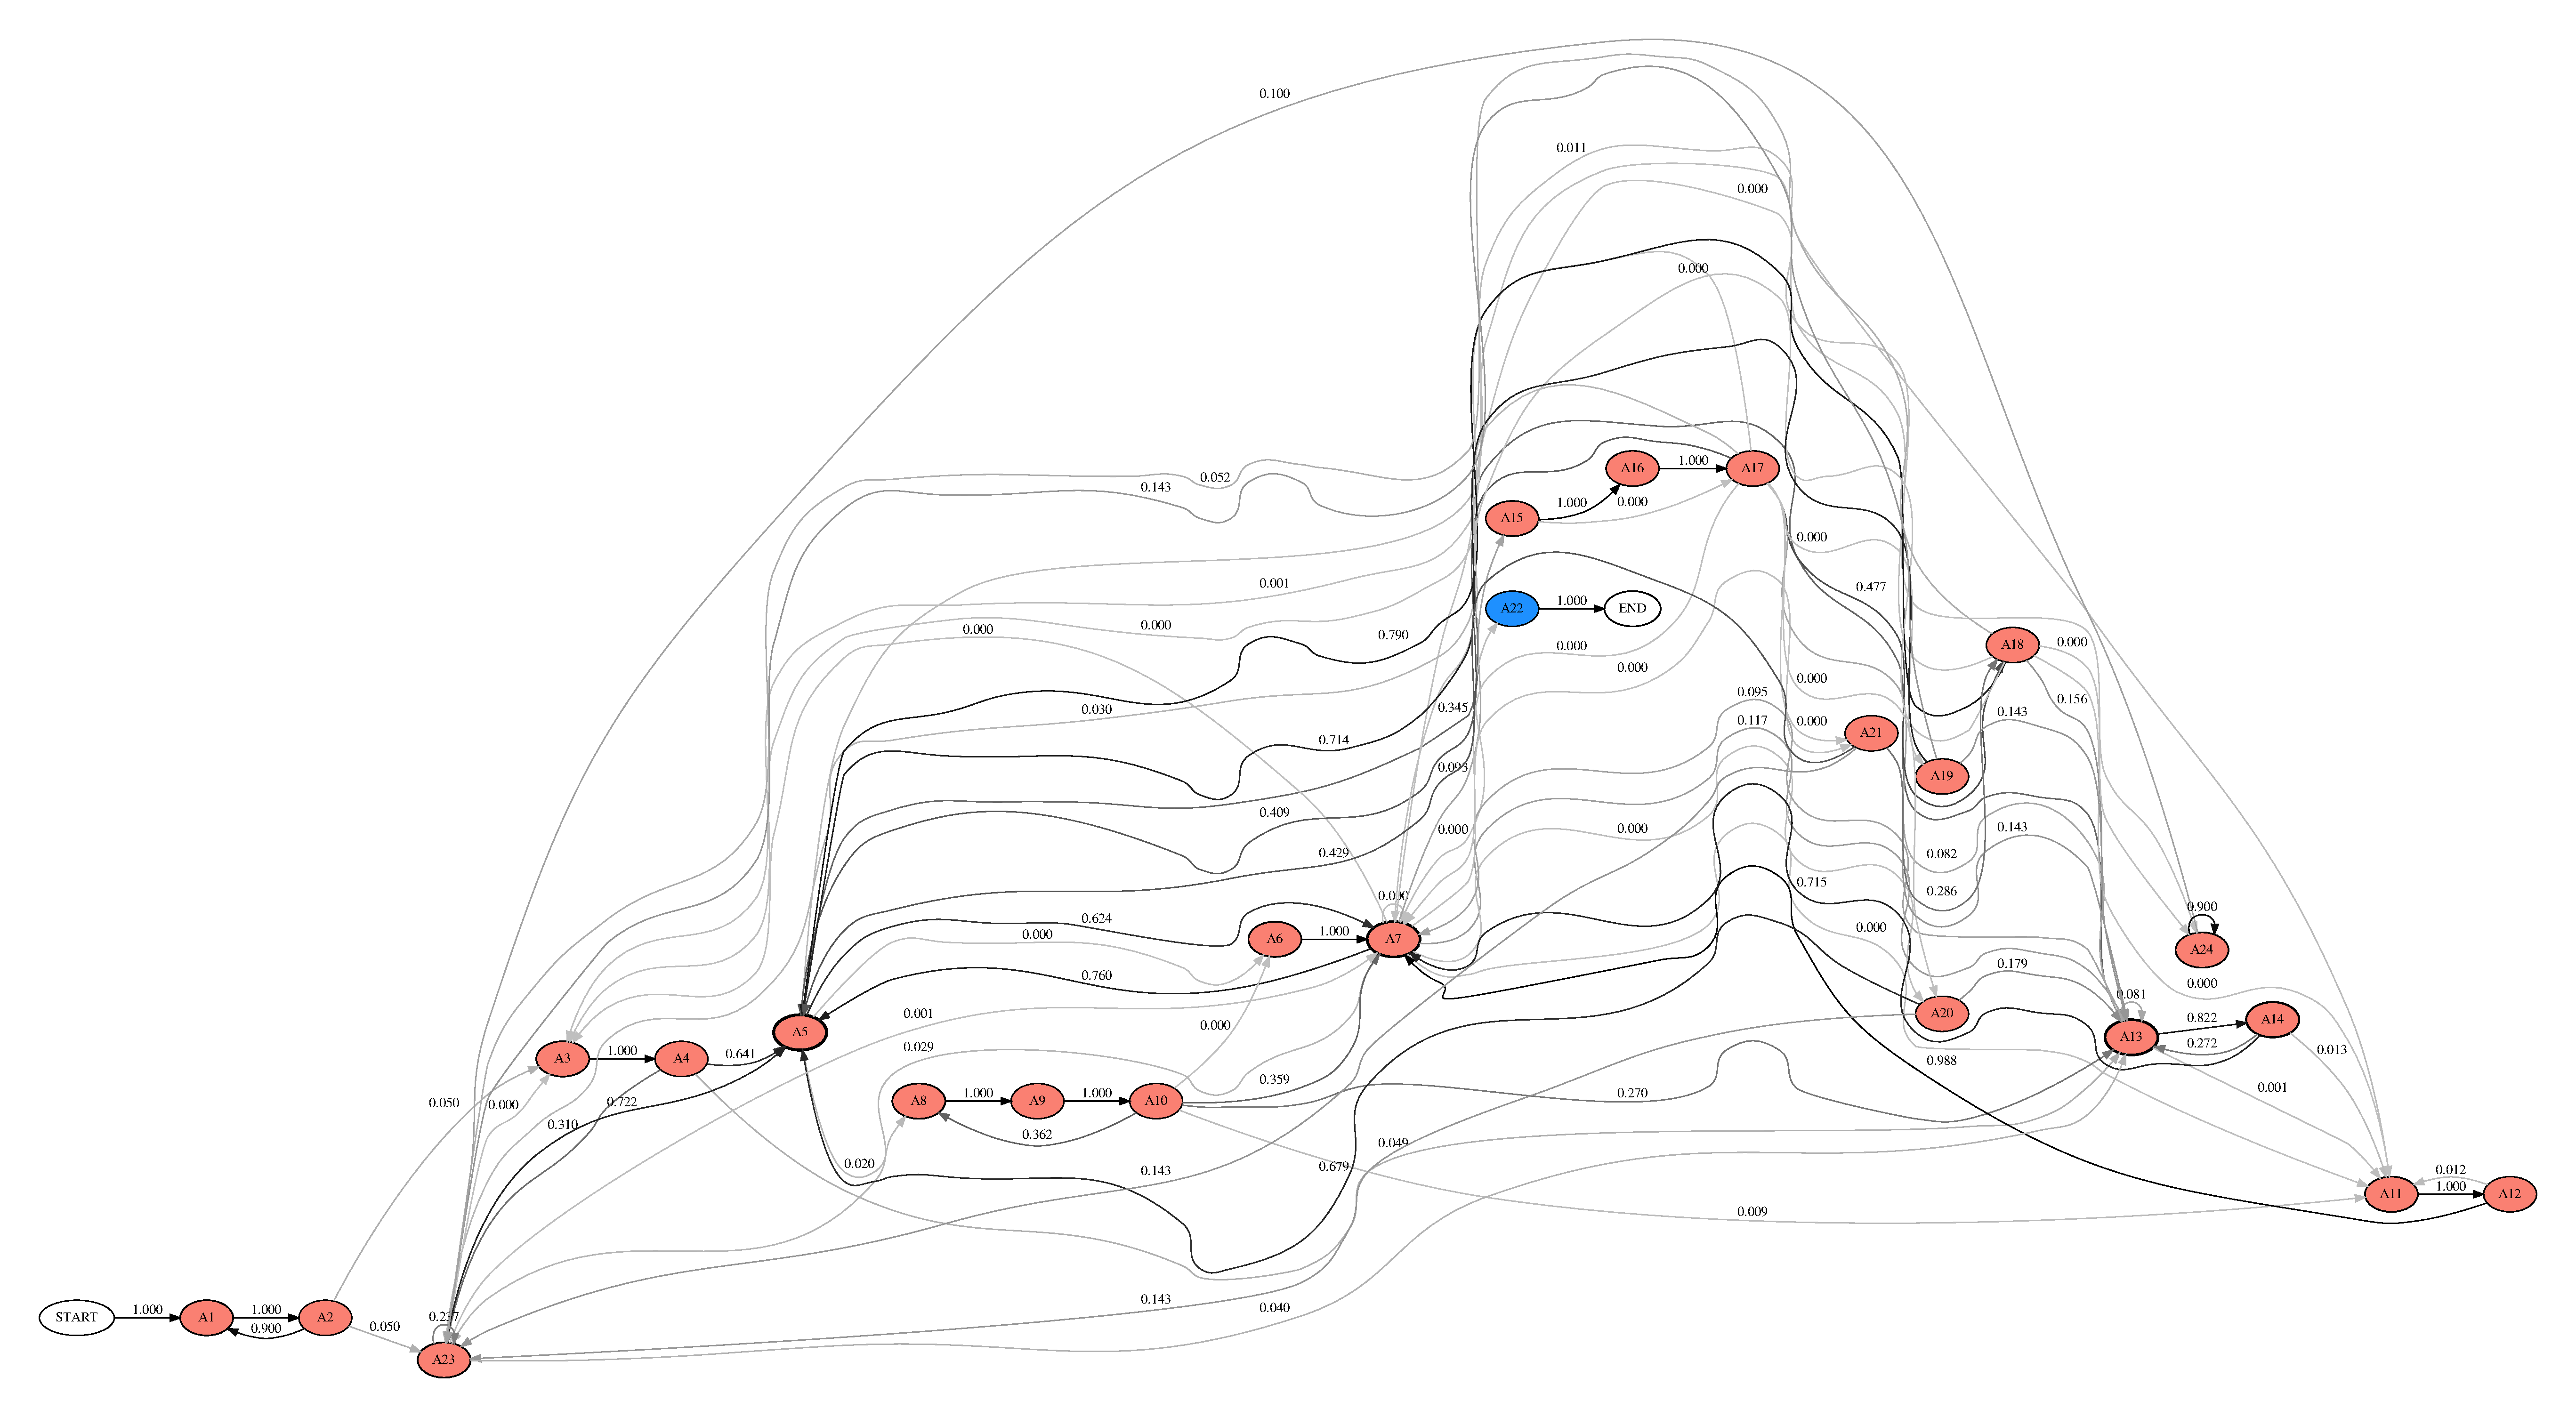
\includegraphics[width=0.35\textwidth]{../plots/mpenny-pop10/mpenny_10.pdf}
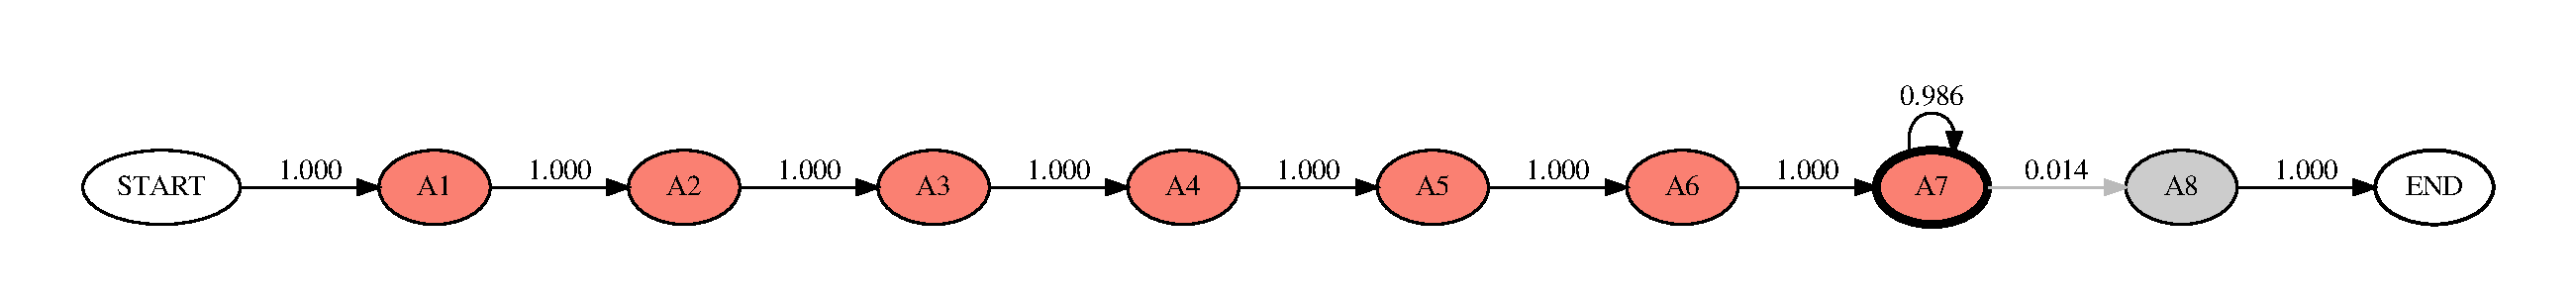
\includegraphics[width=0.40\textwidth]{../plots/model_lambda/model_posterior.pdf}
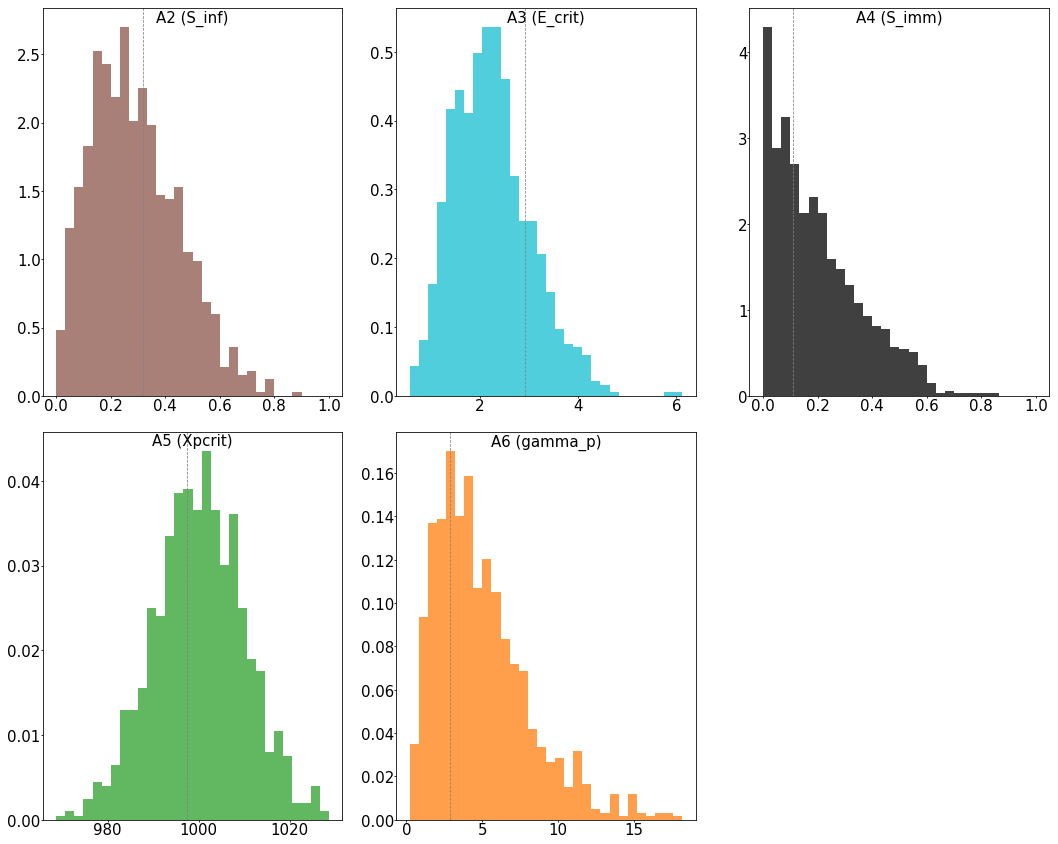
\includegraphics[width=0.40\textwidth]{../plots/model_lambda/hist_posteriors.png}
% \vspace{-10pt}
\caption{An example of the posterior output of population-based simulator after hijacking. \textit{Top}: Represents the posterior execution traces of the simulator, inside the the probabilistic programming 
system. Each address $A_{i}$ correspond to a physical process within the simulator, we describe these addresses and their structures in more details in Section~\ref{sec:casestudy}.
\textit{Bottom}: Represents the histograms generated after posterior inference for the parameters of interest, in this case those parameters are represented by addresses $A_{2}$ to $A_{6}$, conditioned on some observations. 
The grey dashed lines represent the ground truth.}
\vspace{-25pt}
\label{fig:hijacking} 
\end{wrapfigure}
For all the brilliance of probabilistic programming, if one did want to run an existing simulator in a standard probabilistic programming set-up one would have to entirely re-write the simulator in the language of the PPS.
This in many cases is not feasible, nor efficient due to both the size 
and complexity of the existing simulator code base. 
However, what if one could connect arbitrary a simulator, written in any
language and directly connect it to a PPS, without having to re-write
the simulator in the given PPS?

  
\paragraph{Related work} Our method of hijacking simulators builds on the work of~\cite{baydin2018efficient,casado2017improvements}. 
They demonstrated how this could be done for event-based simulators, but there methods neglected a large class of population-based simulators that model interactions 

between populations, that are utilized for modeling epidemics, multi-agent systems and financial economics \cite{raberto2001agent,landau_binder_2014,hartig2011statistical,smith2008towards,bershteyn2018implementation}. 
Our framework provides a solution and makes it easy to transform arbitrary stochastic population-based simulator, in addition to the event-based simulators, into probabilistic programs, regardless of the complexity of the simulator. 
Our system supports simulators written in 13 different programming languages and enables the user to perform posterior inference over the density of the simulator, conditioned on what data the user has access too, including 
simulator output. 
We provide a theoretical justification for our approach and many examples.
% This enables two things.
% 1) It enables software developers and researchers to understand complicated code bases. 
% 2) It provides interpretable inference results that provide policy makers with predictions that are truly interpretable, in the sense that the end-user, of the inference results understands what physical events led to inference outcome. 
% This is critical in several domains, and is particularly important in the medical domain. We provide examples of both in Section~\textbf{TO ADD REF}.


% In this paper, we introduce a novel method that allows one to shed light on the inner workings of a large class of population-based stochastic simulators. We achieve this by extending the work of \citep{baydin2018efficient} by interpreting such population-based simulators as probabilistic generative models within the framework of universal probabilistic programming (UPP) \cite{le-2016-inference}. To this end, we \emph{hijack} existing simulators by overriding their internal random number generators.  Specifically, by replacing the existing low-level random number generator in a simulator with a call to a purpose-built UPP ``controller'', which can thus control, track and manipulate the stochasticity of the simulator.


% Moreover, though our focus is on hijacking epidemiology simulators, our general approach and framework can be applied more widely to a general class of stochastic simulators.

% In time, we hope our approach will play a critical role in
% bringing recent advancements in probabilistic programming to bear on
% the vast array of existing simulators used throughout the sciences,
% thereby providing wide-ranging impacts across a number of fields.

 % \section{Background}
% \label{sec:backgorund}

% \begin{itemize}
% \item Paragraph on Probabilistic programming
% \item Paragraph on Simulators keep high-level focus on pop sims later
% \item Paragraph on Baydin et al
% \end{itemize}
% In-silico simulators have become a crucial tool in evidence-based decision-making within a large number of disciplines, including statistical physics~\cite{landau_binder_2014}, financial modeling~\cite{jackel2002monte},
% weather prediction~\cite{evensen1994sequential}, epidemiology~\cite{smith2008towards} and many others.
% In many cases, simulation output can augment or even replace real data that may otherwise be costly or even impossible to generate.
% Recent advances in hardware have enabled simulations to model increasingly complex systems.
% Epidemiology studies the prevalence and spreading of diseases across populations. Recent advances in hardware have enabled simulations to model the dynamics of infectious diseases, such as Malaria, in ever greater detail.

% Probabilistic programming~\cite{gordon2014probabilistic,staton2016semantics,kozen1979semantics} 
% can be used to express probabilistic models and consequently perform automated inference these. Once a probabilistic model has been expressed in a probabilistic programming language, a wide range of inference techniques, such as Markov Chain Monte Carlo (MCMC)\cite{geyer1992practical}, Variational Inference~(VI)\cite{wainwright2008graphical} and Deep Neural Networks~(DNN)\cite{Goodfellow:2016:DL:3086952},  can be used by non-experts in an automated fashion. 
 
% \section{Types of Models and Probabilistic Programming Languages}

% To bridge the gap between the statistics and machine learning community to the probabilistic programming community we provide a useful overview to expose our ideas more concretely. 

% Probabilistic programming languages, broadly speaking\footnote{For a more comprehensive overview see \cite{rainforth2017automating}}, can be classfied into three categories, each type of langauge extends a particular model space, enabling an increasingly complex set models to be represented as programs, but in doing so the notion of posterior and what it means to do inference over the model, at least in a stastically traditional sense, can change.
% % \begin{figure}
% % \centering
% % 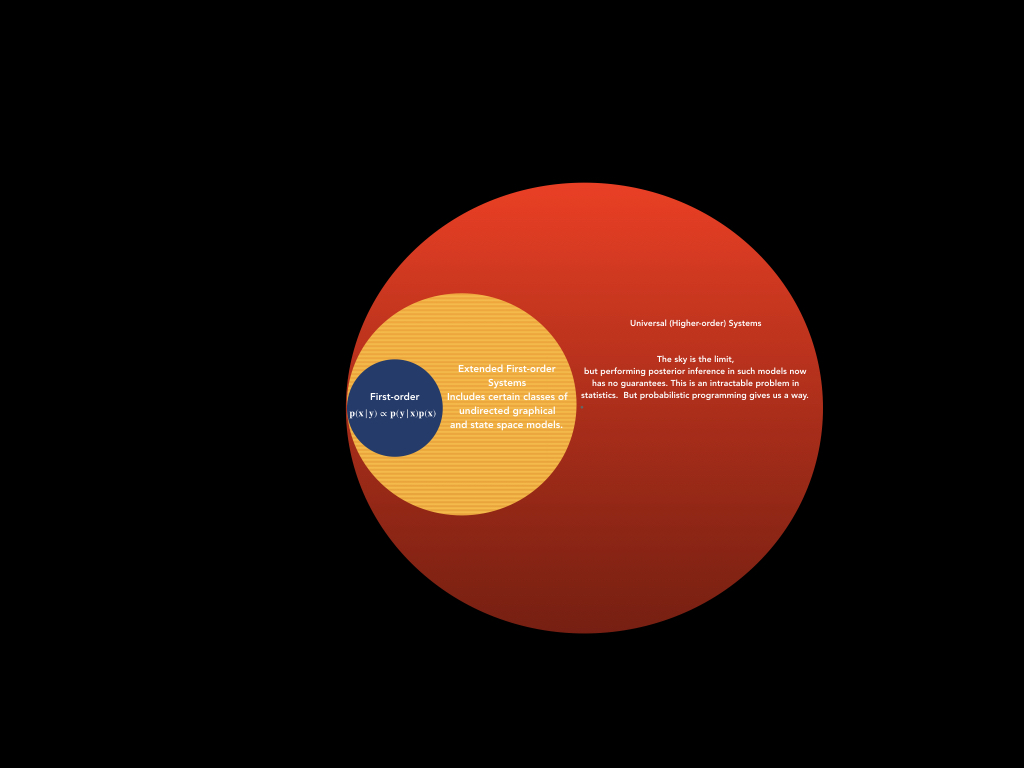
\includegraphics[]{../models/types_of_pp.png}
% % \end{figure}
% The first type of langauges are called first-order languages where the priors are well defined and the \textit{joint} program density constructed via the program directly represent the unormalised stastical joint density $p(x,y)$
% \section{Methodology}
%  TODO


\section{Hijacking Simulators}
\label{sec:methods}
In-silico simulators have become a crucial tool in evidence-based decision-making within a large number of disciplines, including statistical physics~\cite{landau_binder_2014}, financial modeling~\cite{jackel2002monte},
weather prediction~\cite{evensen1994sequential}, epidemiology~\cite{smith2008towards} and many others.
In many cases, simulation output can augment or even replace real data that may otherwise be costly or even impossible to generate.
Recent advances in hardware have enabled simulations to model increasingly complex systems.
Epidemiology studies the prevalence and spreading of diseases across populations. Recent advances in hardware have enabled simulations to model the dynamics of infectious diseases, such as Malaria, in ever greater detail.


\subsection{The Engineering}
Hijacking a simulator a describes the process by which a simulator's random number generators are replaced by calls to external sampling procedures, which are controlled by a probabilistic programming system (PPS). In practice, this amounts to performing a small number of surgical incisions into the simulator's source code in order to replace built-in calls to random number generators. E.g., given a simulator written in C++/Boost\cite{schaling2011boost}, a Gaussian distribution object \textit{boost::normal} is replaced with the corresponding \textit{pyprob\_cpp} distribution object, namely \textit{pyprob\_cpp::distributions::Normal}. Sampling from this distribution is then done by requesting the PPS to send a sample back to the simulator. \bg{This will be extended}


\begin{center}
\begin{tabular}{ |c|c|c| }
\hline
Symbol & Meaning  \\
\hline
\n{x} & Number of latent variables \\
\n{y} & Number of input observations \\
\n{y’} & Number of output observations, generated simulator values \\
\rv{x} & The latent parameters \\
\rv{y} & The input observed parameters \\
\rv{y’} & The output observed parameters \\
\model{\cdot} & Model - i.e .xml file \\
\simu{\cdot} & Simulator \\
\micro{k}{\cdot} & $k$-th Micro-simulation \\
\pdf{\cdot} & probability density function \\
\pmf{\cdot} & probability mass function \\
\add{i} & Address $i$ \\
\expect{\cdot} & Expectation (first moment) \\
\trace{j} & The $j$-th collapsed Trace \\
\traces{i}{j} & A single, un-collapsed Trace for the $i$th trace. ``A program trace’' \\
\stoc{h}{i} & A stochastic process at step $h$ for \add{i} \\
\hline
\end{tabular}
\end{center}
  \begin{algorithm}
  \small
   \caption{Hijacking a stochastic simulator for an arbitrary machine}
    \begin{algorithmic}\small
      \Function{Simulator to a Probabilistic Program}{Simulator $\Omega(\cdot)$, Model input to simulator \model{\cdot}, PPS sampling primitive $f_t()$, Message passing protocol (PPX) $h_t()$, Random variable $x_{sim}$, PPS $\mathcal{P}$ }
       \State  $ x_{sim} \rightarrow f_{t}(x_{sim}) $\Comment{Replace raw sample statements}
       \State $\simu{f_{t}(x^{t}_{sim})} \rightarrow  h_{t}(\simu{f_{t}(x^{t}_{sim})}) \rightarrow \mathcal{P}(f_{t}(x^{t}_{sim}))$ \Comment{An API between the simulator enables raw RNG to be passed through the PPS}
        
        \Function{Create Containerized Environment}{$C(\Delta)$}
        \For{$\delta$ in $\Delta$}
        \State Add dependency $\delta$
        \EndFor
        \State Run Program
       \EndFunction
       \Function{Create thin wrapper}{$f_{t}(x_{t} | \eta_{t})$}
       \State to add
       \EndFunction
       \Function{Create Containerized Environment }{$\Delta_{i}$}\Comment{Where $\Delta_{i}$ is one of $i$-th dependencies}
       \State to add
       \EndFunction
       \EndFunction


\end{algorithmic}
\end{algorithm}


% Stochastic simulators are common across a number of domains, statistical physics~\cite{landau_binder_2014}, financial modeling~\cite{jackel2002monte},
% weather prediction~\cite{evensen1994sequential}, epidemiology~\cite{smith2008towards} and many others. 
% An advantage of using stochastic simulators is that they provide a level of interpretability not found in modern deep learning settings, as they directly incorporate model structure from carefully reasoned observations and experiments. In addition to this, 



The PPS and the simulator exchange xTensor objects \url{https://xtensor.readthedocs.io/en/latest/} through TCP or ICP using a generic FlatBuffers \url{http://google.github.io/flatbuffers/} protocol. On the PPS side, sampling is done using the deep learning framework PyTorch \cite{paszke2017automatic}.

After a variable has been sampled, it is sent to the PPS using \textit{pyprob\_cpp::sample}, alongside with its simulator source trace. This allows the PPS to construct sample trace probabilities and other summary statistics (cf. Section \ref{sec:casestudy}). 

Finally, the entry point to the simulator, i.e. \textit{main} in C++, is replaced by a special \textit{forward} call, in this case \textit{pyprob\_cpp::forward}.
This allows the PPS to generate rollouts from the simulator remotely. 

\paragraph{Population-based simulators} In contrast to the setup used by \cite{baydin2018efficient}, who interface a particle physics simulator that creates a single trace per \textit{forward} call, a population-based simulator creates a trace per population member. This means that e.g. in EMOD, a standard scenario simulation rollout over the span of $3$ years  
with a population of size $n=5000$ \cite{smith2008towards} will generate about \textit{four terabytes} of raw trace data. Unlike with \citep{baydin2018efficient}, this amount of data cannot possibly be kept in RAM, which makes \textit{a posteriori} trace analysis very inefficient. 
In order to deal with the shortcomings of \textit{pyprob} in a population-based simulator context, we therefore extend the framework to be able to do trace analysis on the fly.

By extending \textit{pyprob} to handle population-based simulators, the PPS can now track all stochastic random variables that are created within the simulator, which then allows us to generate trace plots and path probabilities associated to the execution paths of the program.
The corresponding increase of simulator transparency helps reinstate much needed trust between policymakers and evidence-based methods.

\subsection{The Theory}

\bg{Tom add theory stuff here}
%As stated previously, Simulators are complex systems and should be viewed as black-boxes, thus deciphering the underlying processes occurring within the simulator facilitates the users understanding of how such a system operates and provides a way of interpreting the outputs in a clear way. In addition to this, when using a simulator to make new inferences a user will often want to condition on the output of the simulator, or any new observations gathered. In the standard simulator framework this is not possible, but in 
%
%Essentially, from the users perspective, our approach can be viewed as follows the user would first select the simulator that they are going to use, for example EMOD, they would then write their model, in the desired simulator, according to the given simulator specification. The user would then run the simulator. Now comes the hijacking. During the forward run of the simulator all sampling calls from the random number generator are directed through the probabilistic programming system~(PPS), which in addition to the standard output of the simulator now generates a series of result summaries and path probabilities, as we demonstrate in Section~\ref{sec:casestudy}.
%
%By connecting with the PPS we track all sampling procedures, which enables us to control the myriad of random variables generated within the simulator. 
%
%In order to overhaul a stochastic simulator like EMOD, or OpenMalaria, we are only required to override the location of the stochastic primitives, i.e. the base operations that generate the stochasticity and randomness within the simulator. 
%We will walk through how this is done for a standard epidemiology simulator, see the flowchart for a pictorial representation of what is happening \bg{add ref to flow chart}.
%
%The initial step first requires one to build a containerized environment, such as Docker~\cite{merkel2014docker} and Singularity~\cite{kurtzer2017singularity}, which enables the simulators to be run on any device, independent of different hardware architectures, removing the requirement for hardware specific machines. 
%The second step requires one to override the stochastic primitives, which requires re-writing aspects of the sampling procedures inside the simulator. 
%This requires zero domain-expertise and only requires one to find where the sampling calls are originated, this can be done with any basic editor search function.
% Such information is typically saved in $\texttt{RANDOM.<filetype>}$, although it may vary slightly between simulators. We now demonstrate this for a uniform primitive.
%
%The third step is generating the protocols, which enable communication between the simulator and probabilistic programming system. 
%For this we extend the existing bridging framework introduced in~\cite{baydin2018efficient}, which is comprised of the Probabilistic Programming eXecution~(PPX) protocols and a light-weight C ++ interface, however the language of this light-weight interface is dependent on whatever the file type of the $\texttt{RANDOM.<filetype>}$ file is. 
%For both OpenMalaria and EMOD, the file is written in C ++.
%In using these protocols a larger class of sampling procedures can be overridden. The PPX protocols work by making use of the flatbuffer protocols\footnote{\url{https://github.com/google/flatbuffers}}, which require a flatbuffers script to be specified, see here for an example of a flatbuffers script\footnote{https://github.com/probprog/ppx/blob/master/ppx.fbs}. Once this is specified the flat buffers script is compiled and automatically constructs the message passing framework between the simulator and the probabilistic programming system. The flatbuffers script is simple, clean and intuitive, making it easy for a non-expert to produced.
%The next steps requires modifying the $\texttt{main}$ function in $\texttt{main.cpp}$ and defining an additional forward function which runs one execution of the simulator to enable message passing between the simulator and PPS\footnote{A link to an example will be provided after the review period to preserve anonymity}.
%The final step is to create a light-weight interface. As both the EMOD and OpenMalaria are solely based on C ++ we can extend an existing interface called pyprob\_cpp\footnote{\url{https://github.com/probprog/pyprob_cpp}} to account for the additional sampling procedures.
%Once these steps are complete, the containerized environment will now contain everything required to pass models through to the simulators, encode the simulator into a probabilistic program, which can then be evaluated in the PPS.



 %Our method of overriding simulators builds on the work of~\cite{baydin2018efficient} and extends the framework to encapsulate a more diverse range of simulators, in particular population based simulators such as those found in epidemiology.
%Our framework provides a simple solution to do this and makes it easy to transform arbitrary stochastic simulators into probabilistic programs, regardless of the complexity of the simulator and the language that the simulator is written in. 
%In particular, the framework currently supports 13 popular languages, but there is nothing to stop this being extended to any language of interest. 
%Furthermore, we can understand the structure of simulators as programs for both decoding \emph{black-box structures} and for posterior inference, which enables two things. 
%1) It enables software developers and policy makers to understand complicated code bases and dissect the outputs of simulators for guiding policy decision making.
 %2) It provides interpretable inference results that provide policy makers with predictions that are truly interpretable, in the sense that the end-user of the inference results understands what physical events led to the inference outcome. 
 %This is critical in several domains, especially in epidemiology. 
 %We provide examples of (1) in next Section~\ref{sec:casestudy} and discuss the latter in future work as extensions to the the current framework.

\section{Experiments}
\subsection{Epidemiology Simulators}

Malaria epidemiology is governed by a complex set of drivers, 
few of which can be understood in isolation \cite{cameron2015defining,autino_epidemiology_2012,smith2008towards,bershteyn2018implementation}.
These include within-host dynamics, population-specific traits and even local geography.
Comprehensive modeling of all of these components remains challenging, particularly in a region-specific context. 
Computational epidemiology simulators have to reflect these complexities and are usually stochastic in nature. This can make simulation output highly non-trivial to interpret, particularly when trying to draw desired inferences coupled with observed data \cite{mwendera_challenges_2019,ferris_openmalaria_2015}.

We first demonstrate our system on a reduced version of the OpenMalria simulator, proposed by Smith et .al~\cite{smith2006relationship}. The following model directly models the relationship between the entomological inoculation rate and the force of infection for the \emph{plasmodium flaciprum} Malaria. 

Two the most advanced Malaria simulators, namely EMOD~\cite{bershteyn2018implementation} and OpenMalaria  \cite{smith2008towards}, have proven to be particularly valuable to policymakers.
OpenMalaria is based on microsimulations of Plasmodium falciparum in humans and was originally developed to simulate the impacts of malaria vaccines within simple villages or districts
Compared with OpenMalaria, EMOD is able to simulate a variety of additional drivers, including complex geographies complete with migration and a large number of policy interventions
Both EMOD and OpenMalaria are open source and implemented in C++.

\bg{Add linking stuff now to the toy-example where hopefully we can perform inference and }


% Simulators provide users with the ability to model complex environments and problems in a black-box way, enabling new insights to be generated and predictions to be made. A simulator typically encodes several years, if not decades, of research and development and so by their very nature are structurally complicated. 


% Within the context of epidemiology simulators we can model the treatment, infection and prevention cycle under a variety of different environmental conditions, enabling predictions to be made on a set of field observations. Such scenarios in practices would be 


% This enables practitioners to model a wide array of different scenarios at ease.
% However, since the development happens over several years, or decades, usually without comprehensive documentation, understanding a code base written with legacy libraries and software is incredibly difficult and an almost impossible task for a non-expert, or expert who has not had access to the previous years of development. 
%

% Two prominent simulators for modeling Malaria are OpenMalaria~\cite{smith2008towards} and Emod~\cite{bershteyn2018implementation}, which are used by practitioners to model several aspects of the Malaria disease.

%  \paragraph*{OpenMalaria} 
% is an open-source simulator funded by the Gates Foundation to model different aspects of the malaria prevention and treatment cycle for varying population dynamics.
%  Users specify models in OpenMalaria via a scenario file, in the form of an XML document, which determines the specifics of a particular treatment, or prevention strategy, climatic factors, the demographics of the population and so forth. In addition to this, field observations can be encoded inside of, or externally to the scenario file. 
% The scenario file encodes all input and output parameters, some of which we wish to simulate, others remain fixed. 

% \paragraph{EMOD} provides the modularity and structural flexibility necessary for modeling multiple infectious diseases at the within-host and population level. 
% EMOD can be used to model HIV, Tuberculosis, Malaria and generic diseases, but for the purposes of the comparison, we just focus on Malaria. 
% To specify models in EMOD a configuration file is written by the user, which is in the form of a JSON and provides similar functionality to OpenMalaria, in terms of what can be specified and the outputs that it produces. 


% In both these well used simulators users are accustomed to writing their models as either XML, or JSON files and so it is important that any system built around this framework enables the models to be inputted in the same format, without requiring the users to learn how to use a new set of protocols. Our system facilitates this as we shall discuss in the proceeding sections.  

 

\begin{figure}
  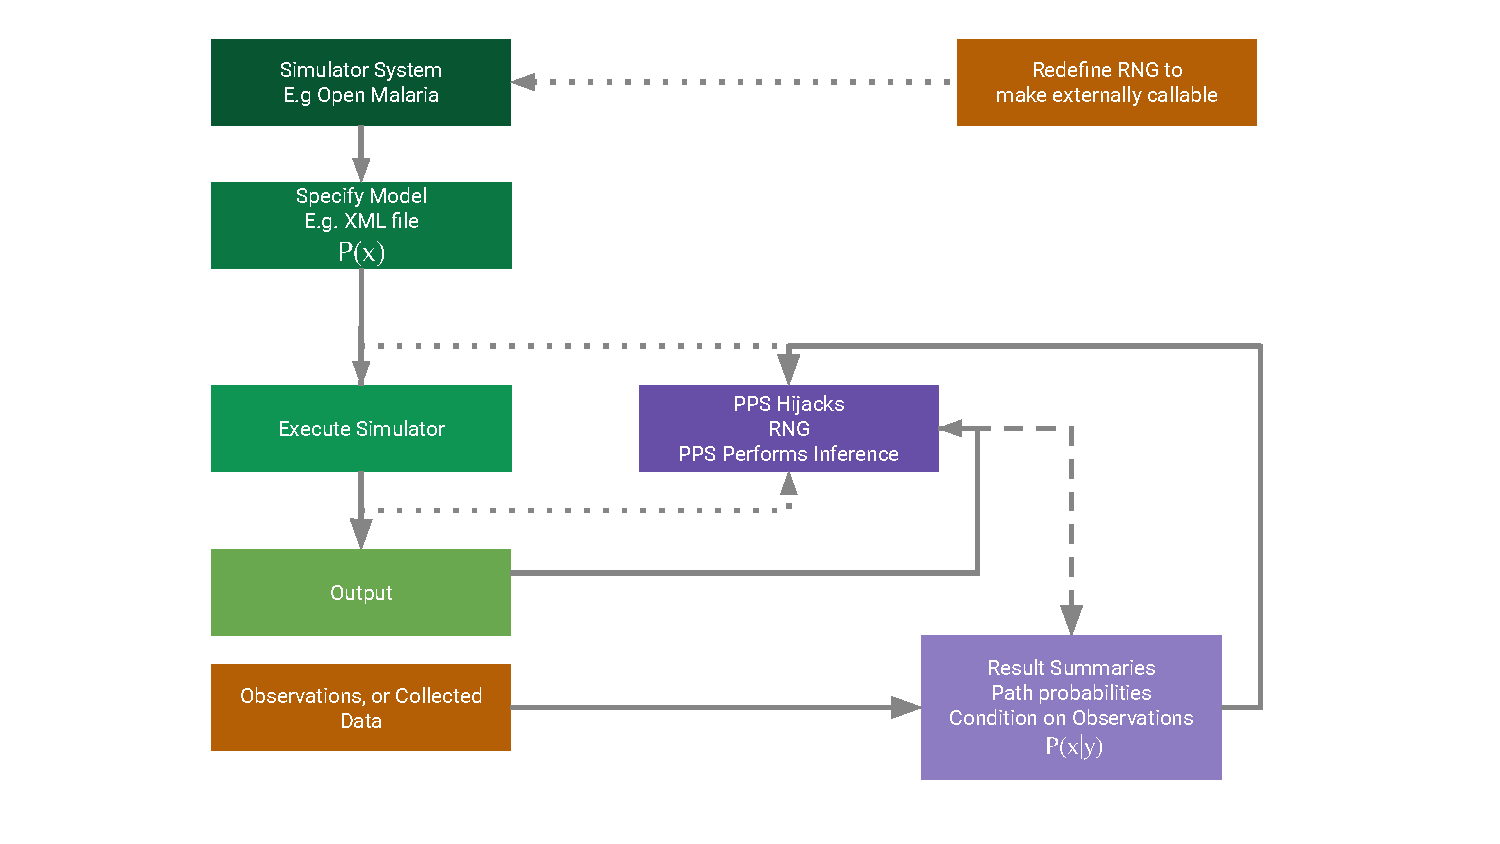
\includegraphics[width=\textwidth]{../plots/system.pdf}
  \label{fig:how}
  \caption{This flow-chart provides an overview of the process of how our system hijacks a generic population-based epidemiology simulator, such as EMOD, and how we modify the simulator to 
  to hijack the random number generator (RNG).}

  \end{figure}


% \begin{table}[h!]
% \footnotesize
% \begin{tabular}{p{3.6cm}|p{3.6cm}}
% Before  &  After  \\
% \midrule
% \begin{lstlisting}
% #include <gsl/gsl_cdf.h>
% #include <gsl/gsl_rng.h>
% #include <gsl/gsl_randist.h>
% //preamble
% double random::uniform_01 () {
%     double result =
% # ifdef 
% OM_RANDOM_USE_BOOST
%        rng_uniform01 ();
% # else
%  gsl_rng_uniform (rng.gsl_generator);
% # endif
%     return result;
%     }
% \end{lstlisting}&
% \begin{lstlisting}
% #include <pyprob_cpp.h>
% #include "xtensor/xadapt.hpp"
% // preamble
% double random::uniform_01 () {
% auto uniform = pyprob_cpp::distributions::Uniform(0,1);
% return pyprob_cpp::sample(uniform)(0);
% }
% \end{lstlisting}
% \end{tabular} 
% \end{table}
% As can be seen, writing the new sampling call is cleaner and syntactically simpler. 
%\bg{Add performance plot showing memory consumptions of pyprob and our new system.}
\subsection{Real-world Example}
\label{sec:casestudy}

\bg{Chris will write up}
Ensemble methods are commonly used in statistics in order to combine the predictive power of multiple models \cite{cameron2015defining,smith_ensemble_2012}. To this end, recent work has attempted to characterise the similarities and differences between two of the most advanced Malaria epidemiology simulators, EMOD \cite{bershteyn2018implementation} and OpenMalaria \cite{smith2008towards}. Evaluation is usually done by comparing a number of output parameters across a range of hand-crafted standard scenarios reflecting different geographical locations across Africa~\cite{smith_ensemble_2012}.

In the following, we illustrate how our method introduces a novel introspection paradigm. By extracting trace graphs from population-based simulators, policymakers can ask specific questions about properties of the model trace flow. 

To illustrate the above, we present simulation output generated from a scenario resembling local conditions in the town of Ifakara (Tanzania). Both EMOD and OpenMalaria are configured to simulate a single population node of $n=100$ and assume constant climatic conditions and no migration over the simulation period of $3$ years. Please refer to Figure \ref{fig:EIR} for the seasonal Entomological Inoculation Rate (EIR), a measure of infectivity.

\begin{figure}[h!]
  \centering
  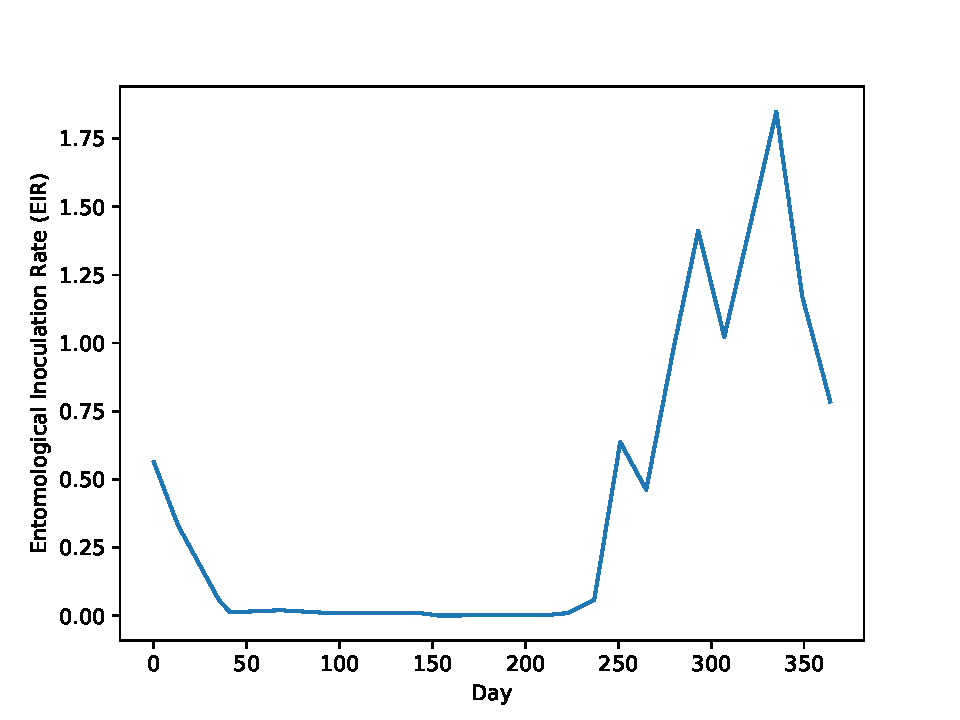
\includegraphics[width=\textwidth/2]{../plots/EIR_Ifakara.pdf}
  \caption{Seasonal Entomological Inoculation Rate (EIR) for the Ifakara scenario. Data is averaged over $30$ day periods.}
  \label{fig:EIR}
\end{figure}

We provide examples of the generated trace plots from the connection between the simulator and the PPS in Figure~\ref{fig:plotewan}. 

We can see from the addressing schemes $A_1, \ldots, A_N$ (Tables \ref{table:addresses} and \ref{table:asingleaddress}) what physical events are connected to each other and how outputs in EMOD are generated from a different set of procedures as compared to OpenMalaria 
By having access to such diagrams users can internally evaluate and scrutinize the decisions that the simulator is making.

This is important for policymakers, or general non-experts, as it not only details how we arrive at the given outputs, but it provides an understanding of which processes were most crucial in determining those outputs as can be seen from the path probabilities assigned to each of the vertices. 

Additionally, by associating nodes in trace graphs representing the same physical processes within different models, the significance of model detail can be evaluated. For example, the full trace presented in Table \ref{table:asingleaddress} represent a sampling step associated with within-host dynamics of the Malaria parasite \textit{Falciparum} in OpenMalaria node $A1$. The same physical process also occurs in EMOD's trace graph at position $A7$ (see Section \ref{table:addresses}).
Comparisons like these could help developers better control model complexity, and even provide an alternative testing and debugging paradigm.


\subsection{Larger Scale-Simulators: OpenMalaria and EMOD}

\begin{figure*}[h!]
  \centering
  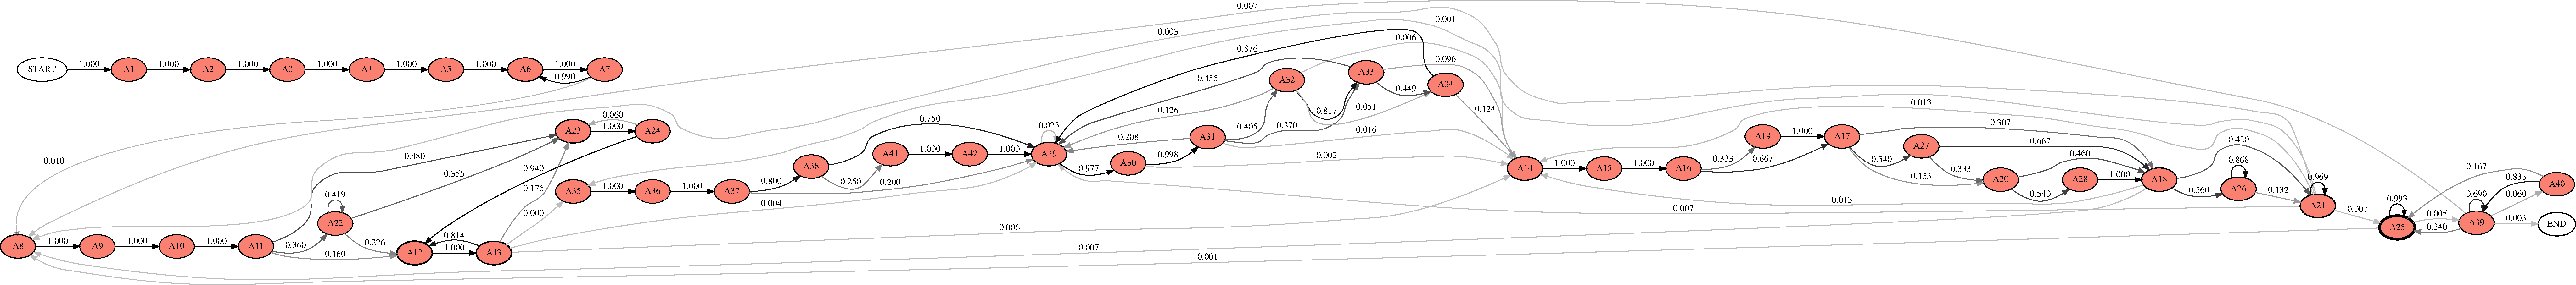
\includegraphics[width=\textwidth]{../plots/final_emod_traces__rotated.pdf}
  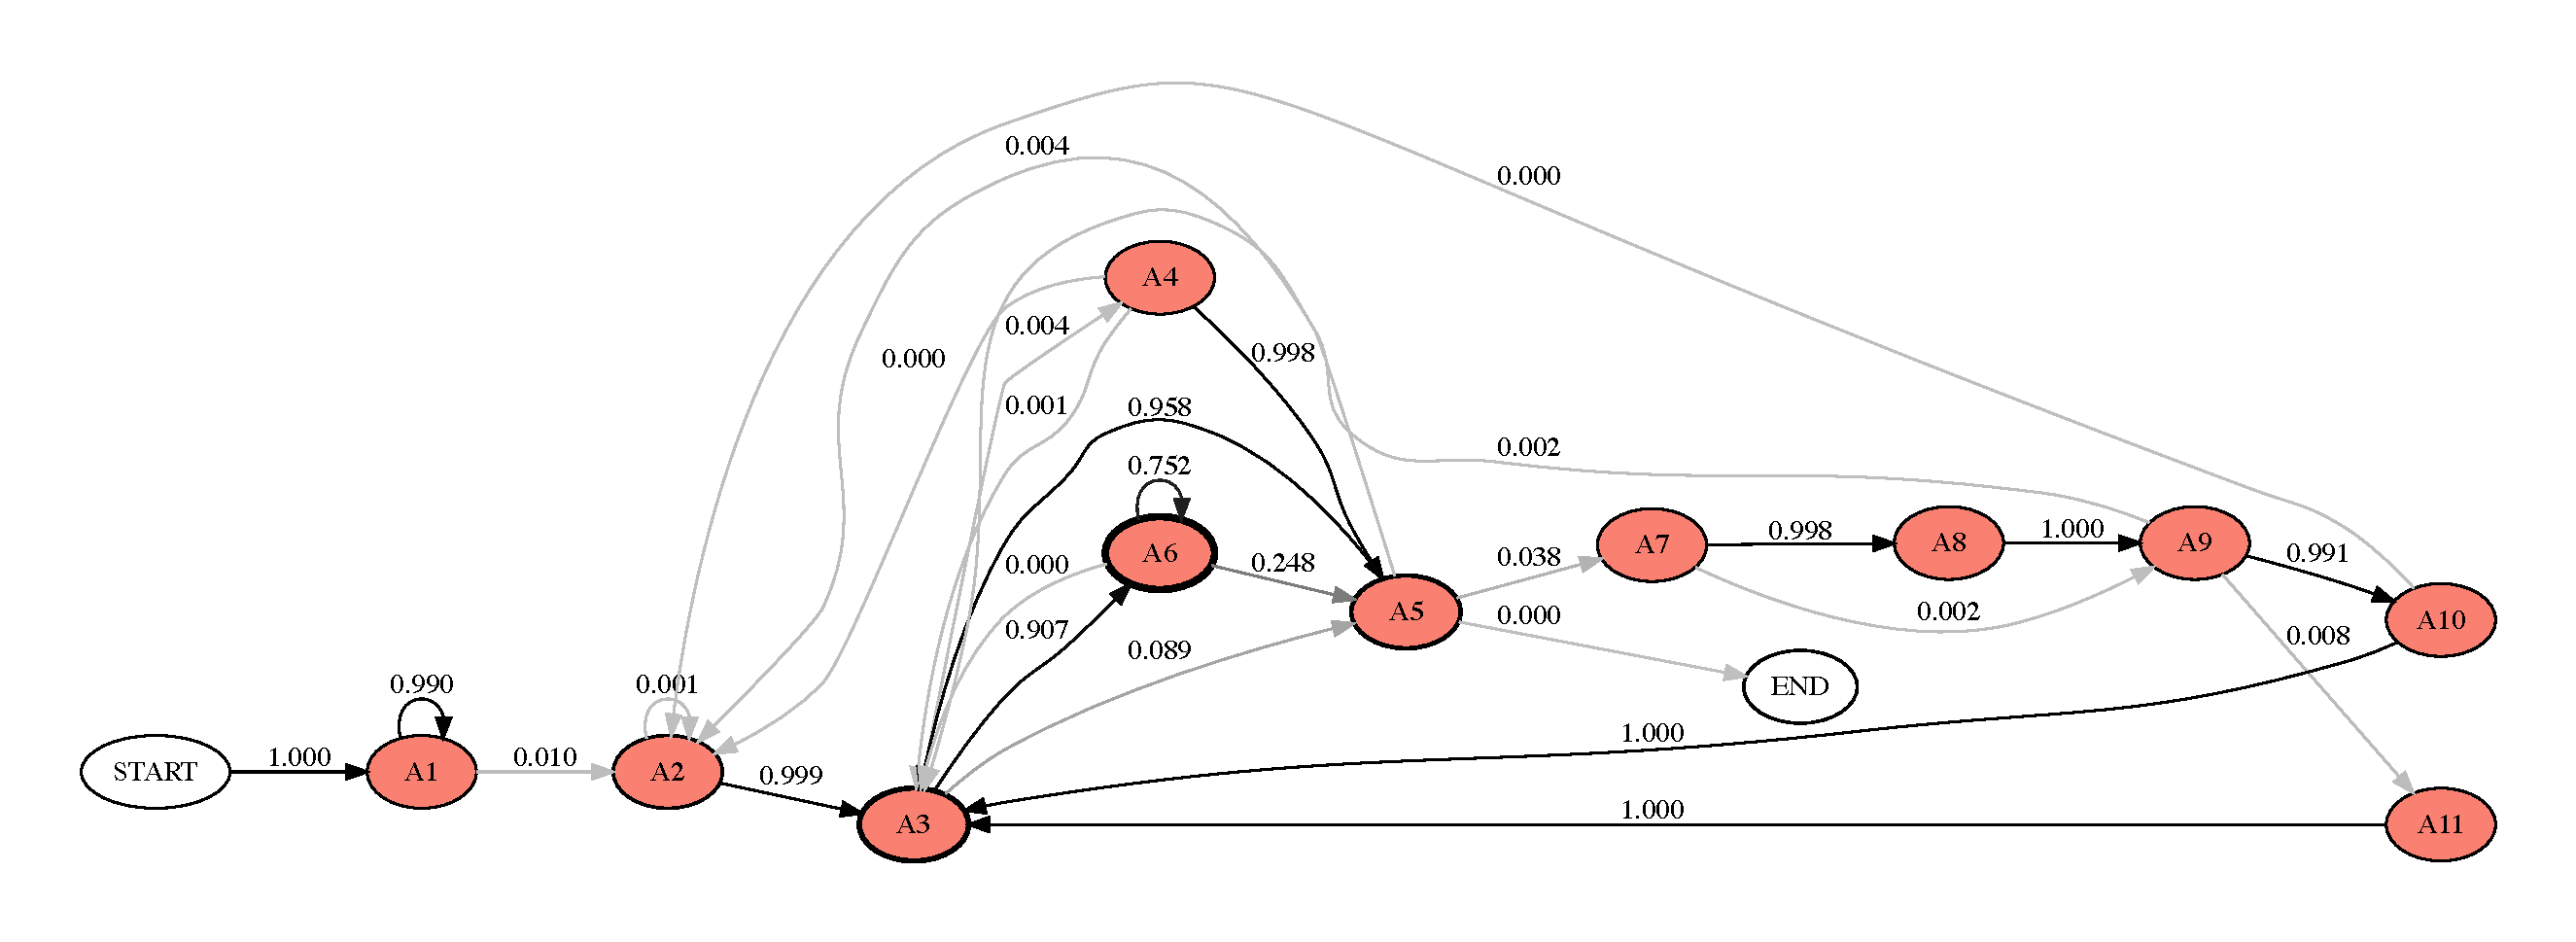
\includegraphics[width=\textwidth]{../plots/ewan_25_pop_100.pdf}
  \caption{Here we run two equivalent models, compare the corresponding trace paths and corresponding 
  path probabilities taken by the thousands of random variables generated internally within the simulators. \textit{\textbf{Top:}} The specified model run in EMOD. \textit{\textbf{Bottom:}} The specified model in OpenMalaria.}
  \label{fig:plotewan}
\end{figure*}

\begin{figure*}
  \centering
  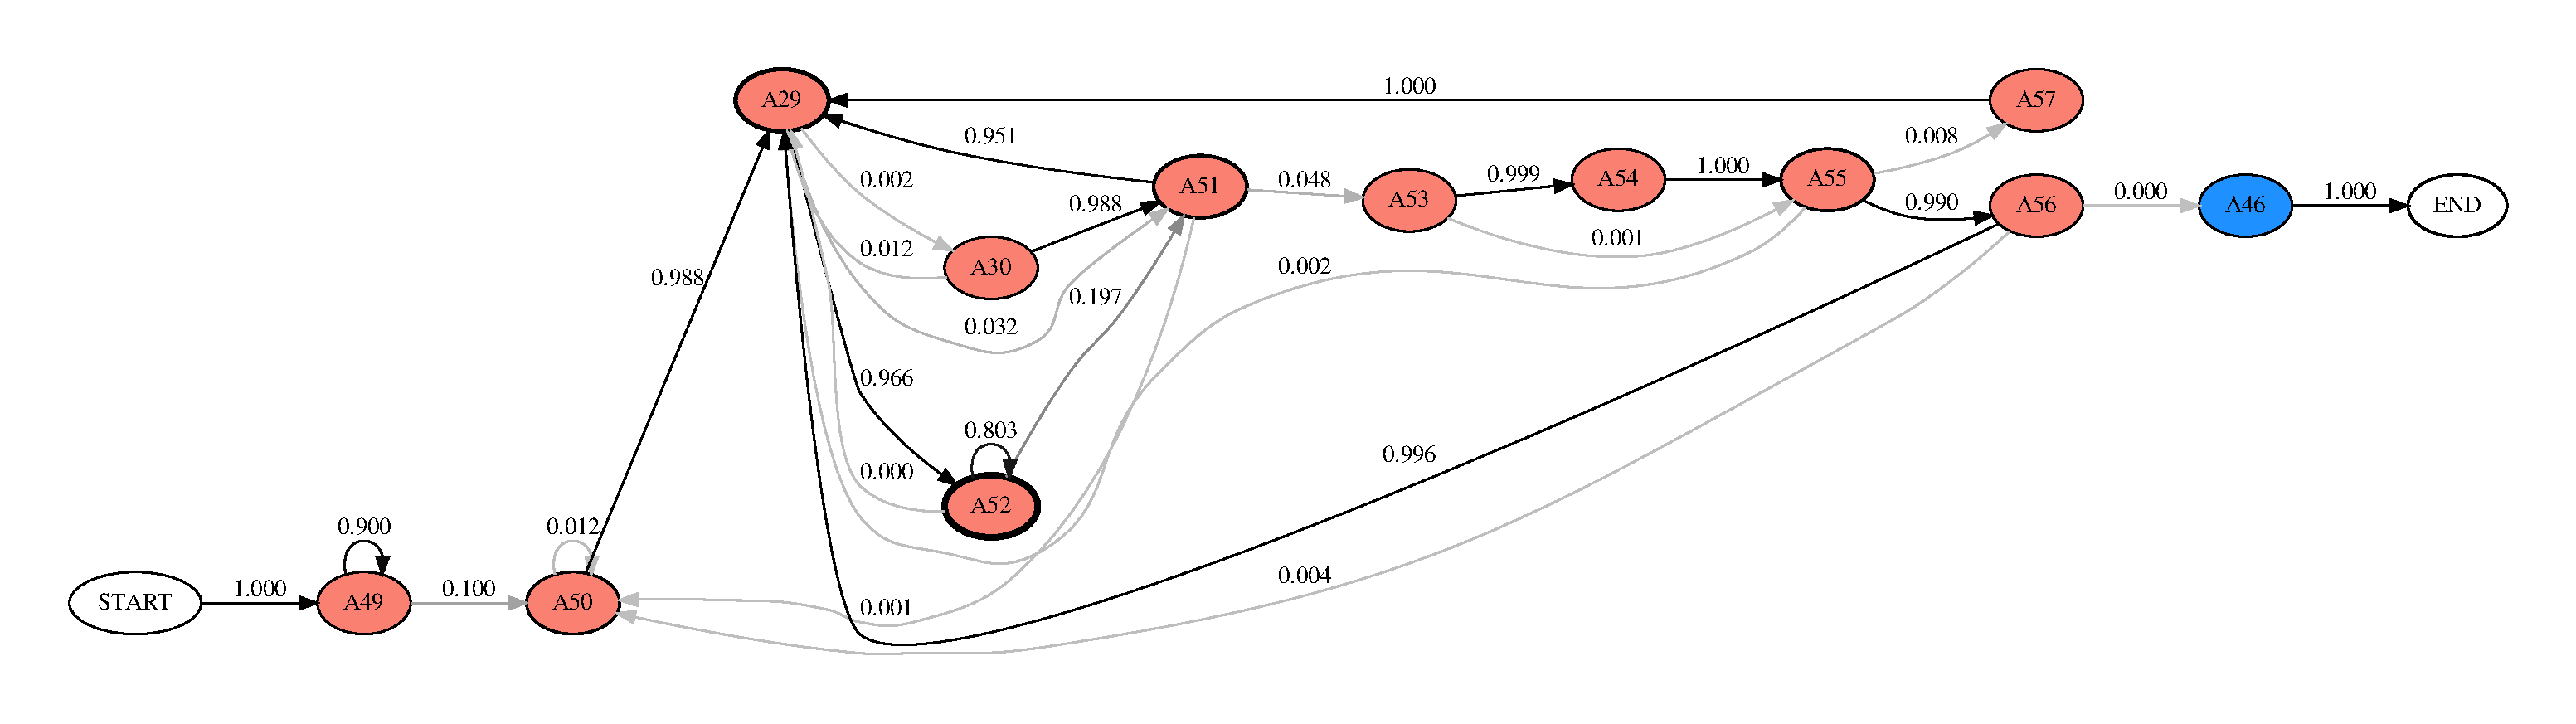
\includegraphics[width=\textwidth]{../plots/mastsari/mastsari_prior_trace_structure.pdf}
  \caption{Prior trace probabilities of the Mastsari model.}
  \label{fig:priortracemastsari}
\end{figure*}

\begin{table}[h!]
\footnotesize
  \setlength{\tabcolsep}{1mm}
\label{table:asingleaddress}
  \caption{An example of an address generated for the model run in the OpenMalaria simulator. We can see that A1
  relates to Generating a member of the human population who may or may not be infect with the Malaria disease. We get something similar for EMOD, except this relates to A7 in the EMOD program execution.}
  \def\arraystretch{1.25}
  % \setlength{\tabcolsep}{1mm}
  \begin{tabularx}{\textwidth}{@{}lX@{}l@{}} 
    \toprule
    Address ID & Full address \\
    \midrule
  A1 & [forward()+0x204;OM::Simulator::start(scnXml::Monitoringconst)+0x28a;
  OM::Population::createInitialHumans()+0x94;

  OM::Population::newHuman(OM::SimTime)+0x5c;
  OM::Host::Human::Human(OM::SimTime)+0x12b;

  OM::WithinHost::WHInterface::reateWithinHostModel(double)+0x99;
  OM::WithinHost::DescriptiveWithinHostModel::DescriptiveWithinHostModel(double)+0x3a;
  OM::WithinHost::WHFalciparum::WHFalciparum(double)+0xe6;
  OM::util::random::gauss(double, double)+0xb4]\_\_Normal \\

  $\vdots$ & $\vdots$ \\

  A5 & [forward()+0x204;OM::Simulator::start(scnXml::Monitoringconst\&)+0x468;
  OM::Population::update1(OM::SimTime)+0xff;

  OM::Host::Human::update(bool)+0x2bc;

  OM::Clinical::ClinicalModel::update(OM::Host::Human\&,double, bool)+0x96;

  OM::Host::NeonatalMortality::eventNeonatalMortality()+0x9;

  OM::util::random::uniform\_01()+0xc0]\_\_Uniform\\
  $\vdots$ & $\vdots$ \\

 % $\vdots$ & $\vdots$ \\

\bottomrule
  \end{tabularx}
  \end{table}

\begin{table}[h!]
  \footnotesize
  \setlength{\tabcolsep}{1mm}
  \caption{An interpretation table for each of the address of the 
  overall trace generated from the corresponding OpenMalaria model.}
  \label{table:addresses}
  % \def\arraystretch{1.25}
  % \setlength{\tabcolsep}{1mm}
  \begin{tabularx}{\textwidth}{@{}lX@{}} 
    \toprule
    Address ID & Interpretation \\
    \midrule
  A1 & Generate a human in the population within host dynamics\\

  
  A2 & Generate another human in the population within host dynamics\\

  A3 & The population is updated and a new human, or humans, may get infected \\

  A4, A5 & Potential child deaths within the population are simulated \\

  A6 & Determines parasite density of an individual infection \\

  A7 & Models how the disease is progressing within the infected humans \\

  A8 & Models how the disease is progressing within the population \\
  
  A9 & Models how the disease is progressing within the infected humans after the population has been updated\\

  A10 & Full clinical update on the population for those without severe or no Malaria infection. \\

  A11 & Full clinical update on the population for those with severe Malaria infections \\
\bottomrule
  \end{tabularx}
  \end{table}


\section{Discussions and Future Work}

In this work we have demonstrated a method 
that enables one to hijack populationbased simulators, extending 
the work of \citep{baydin2018efficient}. 
We applied our method to two Malaria orientated population-based simulators and 
generated a variety of trace graphs.
Finally, we have shown how our system
enables policy makers and non-experts to analyse simulator outputs in a 
way previously unavailable in the field of epidemiology. 

To extend our work further we aim to implement additional 
tools that will facilitate complicated inference procedures that condition on simulator 
output. We will also evaluate additional scenarios across Africa and South-East Asia to better understand the similarities and differences between EMOD and OpenMalaria.


% \subsubsection*{Acknowledgments}

% Use unnumbered third level headings for the acknowledgments. All acknowledgments
% go at the end of the paper. Do not include acknowledgments in the anonymized
% submission, only in the final paper.

% \section*{References}

\bibliographystyle{plain}
\bibliography{refs,malaria}

\end{document}